\scanpage{6}
\[
\begin{aligned}
(P/Q)'&=\frac{P'}{Q}-P\frac{Q'}{Q^2}=\frac{P'Q-Q'P}{Q^2}\\
(P/Q)''&=P''/Q\deleted{\unsure{+}}\unsure{-|+}2\frac{P'Q'}{Q^2}+\deleted{\unsure{2}}P\bigl(
\end{aligned}
\]
\[
\frac{P'}{\deleted{Q}P}-\frac{Q'}{Q}
\qquad (xy)^{\unsure{2|''}}=\unsure{x''|x^2}y+2x'y^{\unsure{\prime}}+xy^{\unsure{\prime\prime|\prime}}
\]
\[
\left(\frac{\deleted{\unsure{P'}}f}{g}\right)'=\frac{f'g-g'f}{g^2}
\]
\[
\frac{(P''Q+\deleted{P'Q'}-\deleted{P'Q'}\deleted{\unsure{+}}\unsure{-|+}Q''P)
\unsure{Q^{\deleted{2}}|\deleted{Q}^{\,2}|Q^2}
 -(P'Q-Q'P)2\deleted{Q}Q'}{Q^3}
\]
% The long diagonal meets the raised 2 and the right edge of the preceding Q.
% Its relation to a local cancellation remains uncertain; all visible glyphs are retained above.
% The next fraction bar has a second, lower stroke beneath its right-hand portion.
\figure{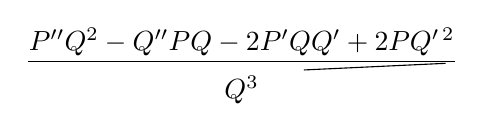
\begin{tikzpicture}
\node[inner sep=0pt,anchor=south west] (num) at (0,0)
 {$P''Q^2-Q''PQ-2P'QQ'+2PQ'^{\,2}$};
\draw ([yshift=-2pt]num.south west)--([yshift=-2pt]num.south east);
\draw ([xshift=3.5cm,yshift=-5pt]num.south west)--([xshift=-0.12cm,yshift=-2.6pt]num.south east);
\node[inner sep=0pt,anchor=north,yshift=-7pt] at (num.south) {$Q^3$};
\end{tikzpicture}}
\[
2p^2Q^2\bigl(-\frac{Q'}{Q}+
\]

% Crossed writing in the opposite direction, read after a 180-degree rotation.
% Two long diagonal cancellation strokes cross this complete layer.
\[
\deleted{\det\begin{pmatrix}a\deleted{\unsure{d|b}}&c\\b&d\end{pmatrix}-ad-bc\quad\text{inversible}}
\]
\[
\deleted{\begin{aligned}
&\delta(e_1 e_{d-2})=-e_1\delta(e_{d-2})=-e_1e_{d-3}\deleted{=e_d}\\
&\phantom{\delta(}\rotatebox{90}{$=$}\\
&\delta(a\eta)=a\delta\eta=a\alpha e_{d-2}+a\beta f_{d-2}
\end{aligned}}
\]
\[
\deleted{\begin{aligned}
&\delta(e_1 f_{d-2})=-\deleted{f}e_1\cdot f_{d-3}\\
&\phantom{\delta(}\rotatebox{90}{$=$}\\
&b\alpha e_{d-2}+b\beta f_{d-2}
\end{aligned}}
\]
\[
\deleted{\begin{aligned}
&\delta(f_1 e_{d-2})=\delta(f_1)e_{d-2}-f_1\delta(e_{d-2})=e_{d-2}-f_1e_{d-3}\\
&\phantom{\delta(}\rotatebox{90}{$=$}\\
&\delta(c\eta)=c\delta\eta=c\alpha e_{d-2}+c\beta f_{d-2}
\end{aligned}}
\]
\deleted{etc}

% Detached point at full-scan (968,603), lower-left of On in the rotated orientation.
% Its role, hand, and membership in the cancelled layer are undetermined.
\(\underset{\unsure{\cdot}}{\phantom{O}}\)\deleted{On en tire $e_1e_{d-3}$, $\deleted{\unsure{f}}e_1f_{d-3}$, $f_1e_{d-3}$, $f_1f_{d-3}$ comme comb. lin des $e_{d-1}$ et $f_{d-2}$, à coeff entiers fonctions de $\alpha,\beta$, $a,b,c,d$}

\[
\deleted{\begin{aligned}
&\delta(e_1x_i)=-e_1\delta(x_i)=-e_1\deleted{\unsure{\delta}}x_{i-1}\qquad 2\leq i\leq{}\\
&\phantom{\delta(}\rotatebox{90}{$=$}\\
&\delta(\deleted{\unsure{S}}s e_{i+1}+t f_{i+1})=s e_i+t f_i
\end{aligned}}
\]
% archive sheet number: 5
